	\documentclass[11pt]{article}
%Gummi|063|=)
\title{\textbf{Image Processing}}
\author{}
\date{}
\usepackage{amsmath}
\usepackage{graphicx}
\begin{document}

\maketitle

\section{Abstract}
Our group chose to use our existing knowledge of linear algebra and apply it to the field of linear algebra. We chose to package our end result as a simple python module. Our system can apply linear transformations to the image, rotate, scale. Our system can do convolution based operations, Sobel edge detection, Gauss blur. We also have various color manipulating functions, saturation, brightness, grayscale.

\section{Functionality}
\subsection{Translation Matrix}
For our first feature we implemented various transforms. To do this we first have to express our large image matrix in a way in which we can apply a transformation matrix. When we first import an image we import it as n by m by 3(r,g,b) matrix where n and m are the size of the image. This matrix needs to be converted to a 6 by n*m matrix
$$\begin{pmatrix}
	x & 0 & ...\\
	y & 0 & ...\\
	1 & 1 & ...\\
	r &  255 & ...\\
	g & 255 & ...\\
	b & 255 & ...\\
\end{pmatrix}$$
 With this matrix, One can simply apply a transformation matrix with a 3x3 identity in the lower corner right hand corner. For example a rotation matrix is:
 $\begin{pmatrix} 
	cos(\theta) & -sin(\theta) & 0 & 0 & 0 & 0\\
	sin(\theta) & cos(\theta) & 0 & 0 & 0 & 0\\
	0 & 0 & 1 & 0 & 0 & 0\\
	0 & 0 & 0 & 1 & 0 & 0\\
	0 & 0 & 0 & 0 & 1 & 0\\
	0 & 0 & 0 & 0 & 0 & 1\\
\end{pmatrix}$

A demo translation matrix is:
  $\begin{pmatrix}
	1 & 0 & dx & 0 & 0 & 0\\
	0 & 1 & dy & 0 & 0 & 0\\
	0 & 0 & 1 & 0 & 0 & 0\\
	0 & 0 & 0 & 1 & 0 & 0\\
	0 & 0 & 0 & 0 & 1 & 0\\
	0 & 0 & 0 & 0 & 0 & 1\\
\end{pmatrix}$
where dx and dy are your translation.

Although these transformations work great in this format this is not the format needed to export the image. When doing these transformations, the xy coordinates of each pixel might be mapped to a non integer value. To recreate the image, we must first sample this list and interpolate between points that are close to each pixel in the new image.


\subsection{Flipping}
Another way to do manipulation of an image is via a rotated identity matrix. 

$A = \begin{pmatrix}
	0 & 0 & 0 & 1\\
	0 & 0 & 1 & 0\\
	0 & 1 & 0 & 0\\
	1 & 0 & 0 & 0\\
\end{pmatrix}$

One can then use this to flip an image both vertically and horizontally.
If matrix $P$ is ones image, one can flip horizontally with:
$A P$ and vertically with $P A$. 


\subsection{Gaussian Blur}
A Gaussian function is simply just a normal distributions. This function is defined by:

$$
G(x,y) = \dfrac{1}{2\pi \sigma^2}e^{-\dfrac{x^2+y^2}{2 \sigma^2}}$$

Where sigma is the standard deviation for the curve (how much blur to apply). 

To apply this function to the image we use convolution. Because we are using discrete data, we use a discrete convolution. To do this convolution we need to first choose a kernel size for our Gaussian function. The Gaussian function never goes to zero, it only crouches zero. A kernel that is the size of the image would be ideal, but it is unneeded because values further away from the 0,0 point are very close to zero. For our tests, we used kernel sizes of (5,5) to (21,21). These gave us good results. 

2D convolution can be thought of as super imposing the flipped kernel on top of the image and adding together each entry of the kernel multiplied by the original.
This graphic sums up the process.
\begin{figure}[htp]
\centering
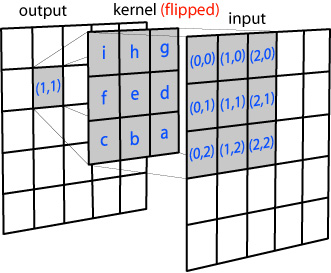
\includegraphics[width=3in]{conv2d_matrix.jpg}
\caption{Convolution in 2D.}
\label{}
\end{figure}

\subsection{Sobel Edge Detection}
Understanding convolution is also quite useful for edge detection. The Sobel operator is technically a discrete differential operator in 2d. Basically we are calculating the gradient for the function. This gradient can be expressed as two kernels. One for the derivative in the x direction and one for the derivative in the y direction. 

Kernel in the X direction:
$\begin{pmatrix}
	-1 & 0 & 1\\
	-2 & 0 & 2\\
	-1 & 0 & 1\\
\end{pmatrix}$

Kernel in the Y direction:
$\begin{pmatrix}
	-1 & -2 & -1\\
	0 & 0 & 0\\
	1 & 2 & 1\\
\end{pmatrix}$
 
One can then take distance $\sqrt(x^2+y^2)$ between these two values, to get the edges. 

Edge detection is simply finding where the rate of change between different colors is quite high so it makes sense to use a differential operator. 

Another interesting thing to note about edge detection is that one can tune how small the edges should be. This can be done by applying a Gaussian blur before this filter.

\subsection{Color Transformation}
Our images are made up of three channels, red, green, and blue. One can manipulate these channels to change how the colors are represented. For example, to output a gray scale, one can simply average all three channels and output 3 of that average.

To increase or decrease the brightness, one can multiply by a some constant. If this constant is greater than one, the image becomes brighter. If it is less, the image becomes darker. 

To invert the image, one can subtract each channel from the max value, in our case, 255.


HUE SATURATION HERE IF POOSSIBLe


\subsection{SVD??}


\section{Conclusion}
More here.... Do we need this section?


\end{document}


%http://www.dreamstime.com/royalty-free-stock-photography-old-european-church-image6109687
%http://amazing-creature.blogspot.com/2011/08/20-cute-bunny-pictures.html


